\documentclass[journal,draftclsnofoot]{IEEEtran} 
\usepackage{graphicx}            %include pictures
\usepackage{amsmath}             %math functions
\usepackage{siunitx}             %fills in si units and order of magnitudes (mm, micro)
\usepackage[hyphens]{url}        %websites, hyphenated when longer than a line
\usepackage{cleveref}
\usepackage{hyperref}
\usepackage{algorithm2e}
%%%%%%%%%%%%%%%%%%%%%%%%%%%%%%%%%%%%%%%%%%%%%%%%%%%%%%%%%%%%%%%%%%%%%%%%%%%%%%%%%%%%%%%%%%%%%%%%%%%%%%%%%%%%%%%%%%%%
\begin{document}
\title{ELEN 4020 Project - Comparison of Parallel Equi-Join using MPI and OpenMP}
\author{Uyanda~Mphunga~-~1168101,~Darren Blanckensee~-~1147279,~Ashraf Omar~-~710435 and~Amprayil~Joel~Oommen~-~843463
\thanks{School of Electrical \& Information Engineering, University of the
Witwatersrand, Private Bag 3, 2050, Johannesburg, South Africa}
}
\maketitle
\pagestyle{plain}
\begin{abstract}

\end{abstract}
%%%%%%%%%%%%%%%%%%%%%%%%%%%%%%%%%%%%%%%%%%%%%%%%%%%%%%%%%%%%%%%%%%%%%%%%%%%%%%%%%%%%%%%%%%%%%%%%%%%%%%%%%%%%%%%%%%%%%
\section{Introduction}
The join operation concerns the combining of two different tuples on a common join attribute \cite{Yu1998}. It is important in information systems, in particular the use of databases since the join operation is the most expensive operation in database query operations in terms of time and data-intensity \cite{Mishra1992}. This project explores two different approaches to performing a join of two very large tables. The purpose of the project are twofold, the primary task is to use parallelism to implement two different join algorithms and the secondary is to compare the algorithms’ efficiency in joining. The problem is described in Section \ref{prob} and the two different approaches discussed in Sections \ref{mpi} and \ref{omp}. The method of experimentation is outlined in Section \ref{desc} and the results of the experiment are analysed in Section \ref{ana}. Section \ref{conc} reviews the project and concludes this document.
%%%%%%%%%%%%%%%%%%%%%%%%%%%%%%%%%%%%%%%%%%%%%%%%%%%%%%%%%%%%%%%%%%%%%%%%%%%%%%%%%%%%%%%%%%%%%%%%%%%%%%%%%%%%%%%%%%%%
\section{Problem Description}\label{prob}
The objective of this project is to perform an equi-join of two very large tables. An equi-join is a type of join that uses the equality operator as a basis for the join \cite{w3resource.com2018} that is if the join attribute in $R_{1}(A,B)$ is strictly equal to the join attribute in $R_{2}(A,C)$ the result of the join is inserted into a third table $R_{3}(A, B, C)$. An illustrated example can be seen in Figure \ref{fig:Equi-Join}.
\begin{figure}[htbp]
	\centering
		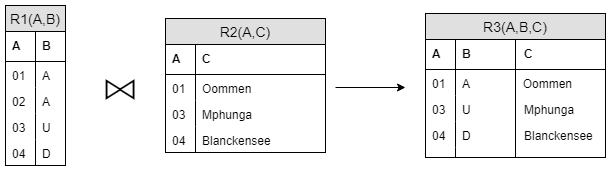
\includegraphics[width=0.4882\textwidth]{Equi-Join.png}
	\caption{An example of equi-join between two relational tables}
	\label{fig:Equi-Join}
\end{figure}
The join must be done using two different algorithms, one that is based in MPI (Message Passing Interface), and one that uses another high-level parallel programming model. The programming model chosen in this project is OpenMP. The two programs need to be compared with one another in terms of speed-up and scalability when increasing the number of processors and nodes that the program uses. The speed-up comparison is performed by running the two programs with increasing number of processors and the scalability comparison is conducted by increasing the number of nodes the program uses in a cluster. Based on the literature, there are multiple join algorithms. The algorithms chosen by the authors are the hash algorithm and the merge algorithm, which form part of the equi-join family of join algorithms and are widely used~\cite{Wolf1993}.

The join algorithms are designed to read data from  file of a specific format and to perform the required operations as per specific algorithm. The algorithms read data of the same file in order to be able to compare their performance. The algorithms are both implemented in C++. This allows for accurate comparisons of the algorithm performances and consequently prevents the possible time lags that may arise from the use of different programming languages. C++ was used instead of C due to the authors finding easier to use C++ under the given time constraints. Another reason that why C++ was found more favourable is that is offers more functionality than C and due to its Object Orientated Design~(OOD) capabilities and the also due to the fact that the authors are familiar with C++. These algorithms were implemented using parallelism.
%%%%%%%%%%%%%%%%%%%%%%%%%%%%%%%%%%%%%%%%%%%%%%%%%%%%%%%%%%%%%%%%%%%%%%%%%%%%%%%%%%%%%%%%%%%%%%%%%%%%%%%%%%%%%%%%%%%%
\section{OpenMP Join Algorithm -- Merge-Join}\label{omp}
The OpenMP join algorithm being implemented is merge-join also known as sort-merge join~\cite{Graefe1994}. The two table are sorted by join attribute. Then the table are scanned and join attributes are compared to one another. For an equi-join, if the join attribute of one entry is strictly equal to the join attribute of the other table's entry, the entries are joined in the output table \cite{Pavlo2017,Graefe1991}. The implemented algorithm assumes that the sorting of the data has already taken place and proceeds to only perform the join algorithm under that assumption.

References~\cite{Wolf1993,Wolf1990} take into account possible errors that may occur due to data skew for the merge join algorithm. According to~\cite{Wolf1993}, data skew can result in some of the processors being over-utilised and others under-utilised. Reference~\cite{Wolf1993} proposes the use of a divide-and-conquer technique as a solution to handle data skew. Reference~\cite{Wolf1990} approaches the issue of data skew in the merge algorithm by adding an extra scheduling phase. The implemented merge join does not take into account the possibility of data skew and instead relies on OpenMP's computational ability to process certain chunks of data and ability to make numerous threads~\cite{Barney2017}. This technique was chosen due to the resources available, namely a cluster, and time constraints.

An overview of the implemented code can be found in Algorithm \ref{algOmp}. The program is implemented in C++ and makes use of OpenMP to implement parallelism. The ``key'' being referred to in this context is the join attribute and the ``values'' are the other two attributes.
\begin{algorithm}
 \KwData{Table $R_{1}(A,B)$, Table $R_{2}(A,C)$}
 \KwResult{$R_{3}(A, B, C)$}
	sort both tables on key\;
	read in keys from each table and store them in vectors\;
 \For{all key-value pairs in each vector}{
		\If{key from $R_{1}$ == key from $R_{2}$}{
			write key-value output to $R_{3}$\;
		}
	}


 \caption{OpenMP Implementation of merge-join}
\label{algOmp}
\end{algorithm}
%%%%%%%%%%%%%%%%%%%%%%%%%%%%%%%%%%%%%%%%%%%%%%%%%%%%%%%%%%%%%%%%%%%%%%%%%%%%%%%%%%%%%%%%%%%%%%%%%%%%%%%%%%%%%%%%%%%%
\section{MPI Join Algorithm -- Hash-Join}\label{mpi}
A hash join can be generalised into two stages~\cite{Keller1991}, the split phase and the join phase~\cite{Kitsuregawa1992}. In the split phase the hash function is used to partition the data into a number of sets and in the join phase each partition is joined and the result is sent to a common table. Hash join algorithms are considered to be the most efficient join algorithms in terms of speed \cite{Mishra1992}. 

The reviewed literature for the hash join is also concerned about data skew. Some of the said literature include references~\cite{Wolf1990,Keller1991} and other documents. Reference~\cite{Wolf1990} addresses the issue of data skew by implementing multiple hash phases along with the use of a heuristic optimisation algorithm in order to isolate skew elements\cite{Wolf1990}.

An overview of the algorithm being used is listed in Algorithm \ref{algMPI}. The program is implemented in C++ and makes use of MPI to send and receive messages between nodes. The hash function simply takes the sum of all the character's ASCII values to produce a unique hash value. As before, the ``key'' being referred to in this context is the join attribute and the ``value'' the other attributes.
\begin{algorithm}
 \KwData{Table $R_{1}(A,B)$, Table $R_{2}(A,C)$}
 \KwResult{$R_{3}(A, B, C)$}
 \For{all key-value pairs in $R_{1}$}{
  read key\;
	calculate hash as sum(ASCII) of key\;
  calculate (hash\%(no. of processes - 1) + 1)\;
 }
send key-value pairs of $R_{1}(A,B)$ to slave nodes in vector\;
\For{all key-value pairs in $R_{2}$}{
  read key\;
	calculate hash as sum(ASCII) of key\;
  calculate (hash\%(no. of processes - 1) + 1)\;//This is to determine which slave node the key-value pair is sent to.
 }
send key-value pairs of $R_{2}(A,C)$ to slave nodes in vector\;
IN EACH SLAVE NODE:\\
\For{all key-value pairs in each vector}{
	\If{key from $R_{1}$ == key from $R_{2}$}{
		write key-value output to $R_{3}$\;
	}
}

 \caption{MPI Implementation of hash-join}
\label{algMPI}
\end{algorithm}

%%%%%%%%%%%%%%%%%%%%%%%%%%%%%%%%%%%%%%%%%%%%%%%%%%%%%%%%%%%%%%%%%%%%%%%%%%%%%%%%%%%%%%%%%%%%%%%%%%%%%%%%%%%%%%%%%%%%
\section{Experiment Description}\label{desc}
%%%%%%%%%%%%%%%%%%%%%%%%%%%%%%%%%%%%%%%%%%%%%%%%%%%%%%%%%%%%%%%%%%%%%%%%%%%%%%%%%%%%%%%%%%%%%%%%%%%%%%%%%%%%%%%%%%%%
\section{Analysis of Results}\label{ana}
%%%%%%%%%%%%%%%%%%%%%%%%%%%%%%%%%%%%%%%%%%%%%%%%%%%%%%%%%%%%%%%%%%%%%%%%%%%%%%%%%%%%%%%%%%%%%%%%%%%%%%%%%%%%%%%%%%%%
\section{Conclusion}\label{conc}
%%%%%%%%%%%%%%%%%%%%%%%%%%%%%%%%%%%%%%%%%%%%%%%%%%%%%%%%%%%%%%%%%%%%%%%%%%%%%%%%%%%%%%%%%%%%%%%%%%%%%%%%%%%%%%%%%%%%%
%REFERENCES
\bibliographystyle{IEEETran}
\bibliography{Ref}
\cleardoublepage
\onecolumn
%%%%%%%%%%%%%%%%%%%%%%%%%%%%%%%%%%%%%%%%%%%%%%%%%%%%%%%%%%%%%%%%%%%%%%%%%%%%%%%%%%%%%%%%%%%%%%%%%%%%%%%%%%%%%%%%%%%%%%
%APPENDIX
%\appendix
%%%%%%%%%%%%%%%%%%%%%%%%%%%%%%%%%%%%%%%%%%%%%%%%%%%%%%%%%%%%%%%%%%%%%%%%%%%%%%%%%%%%%%%%%%%%%%%%%%%%%%%%%%%%%%%%%%%%%%
\end{document}